% Copyright (c) 2025 Quan-feng WU <wuquanfeng@ihep.ac.cn>
% 
% This software is released under the MIT License.
% https://opensource.org/licenses/MIT

% The generated PDF is licensed under CC BY-NC-ND 4.0.
% https://creativecommons.org/licenses/by-nc-nd/4.0/

\documentclass{article}

% \usepackage{amsmath}
\usepackage{amssymb}
\usepackage{authblk}
\usepackage[sorting=none, style=numeric-comp]{biblatex}
    \addbibresource{from_inspirehep.bib}
    \addbibresource{others.bib}
\usepackage{fontawesome5}
\usepackage[a4paper, margin=2cm]{geometry}
\usepackage{graphicx}
\usepackage{minted}
\usepackage{xcolor}
\usepackage[
    colorlinks=true,
    anchorcolor=violet,
    citecolor=orange,
    linkcolor=blue,
    urlcolor=magenta
]{hyperref}
\usepackage[color=violet]{attachfile2}
% \usepackage{mathrsfs}
% \usepackage{mathtools}
\usepackage{pgfplots}
    \pgfplotsset{compat=1.18}
\usepackage{physics}
\usepackage{slashed}
\usepackage{subcaption}
\usepackage{tensor}
\usepackage[compat=1.1.0]{tikz-feynhand}
    \tikzset{graviton/.style={decorate, decoration={snake, amplitude=.4mm, segment length=1.5mm, pre length=.5mm, post length=.5mm}, double}}

\newcommand{\email}[1]{\footnote{E-mail: \href{mailto:#1}{#1}}}
\newcommand{\eg}{\textit{e.g.}}
\newcommand{\etc}{\textit{etc.}}
\newcommand{\ie}{\textit{i.e.}}
\newcommand{\license}{\footnote{This note © 2024 by \href{https://github.com/Fenyutanchan}{Quan-feng WU} is licensed under \href{https://creativecommons.org/licenses/by-nc-nd/4.0/}{CC BY-NC-ND 4.0}. \faCreativeCommons \faCreativeCommonsBy \faCreativeCommonsNc \faCreativeCommonsNd}}

\DeclareDocumentCommand{\githubsrc}{o}{\IfNoValueTF{#1}{\url{https://github.com/Fenyutanchan/amplitude-for-inflaton-reheaton-graviton.git}}{\href{https://github.com/Fenyutanchan/amplitude-for-inflaton-reheaton-graviton/blob/master/#1}{\texttt{#1}}}}

% \DeclareDocumentCommand{\TBA}{o}{\IfNoValueTF{#1}{{\color{red} TBA.}}{{\color{red} TBA: #1}}}
% \DeclareDocumentCommand{\TBD}{o}{\IfNoValueTF{#1}{{\color{red} TBD.}}{{\color{red} TBD: #1}}}

\newcommand{\notsure}[1]{{\color{green!50!black!100!} #1}}

\newcommand{\ee}{\mathrm{e}}
\newcommand{\ii}{\mathrm{i}}

\DeclareDocumentCommand{\twopi}{o}{\IfNoValueTF{#1}{2 \pi}{\qty(2 \pi)^{#1}}}
\DeclareDocumentCommand{\diracdelta}{o}{\IfNoValueTF{#1}{\delta}{\delta^{(#1)}}}
\DeclareDocumentCommand{\twopidelta}{om}{\IfNoValueTF{#1}{\twopi[] \diracdelta}{\twopi[#1] \diracdelta[#1]} \qty(#2)}

\DeclareDocumentCommand{\iM}{o}{\IfNoValueTF{#1}{\ii \calM}{\ii \calM_{#1}}}
\DeclareDocumentCommand{\Msqr}{o}{\IfNoValueTF{#1}{\overline{\abs{\calM}^2}}{\overline{\abs{\calM_{#1}}^2}}}


% \newcommand{\iM}{\ii \calM}
% \newcommand{\Msqr}{\overline{\abs{\calM}^2}}

\DeclareMathOperator{\artanh}{artanh}
\DeclareMathOperator{\diag}{diag}

\newcommand{\GF}{G_\mathrm{F}}
\newcommand{\GN}{G_\mathrm{N}}
\newcommand{\MPl}{M_\mathrm{Pl}}
\newcommand{\kB}{k_\mathrm{B}}
\newcommand{\mPl}{m_\mathrm{Pl}}
\newcommand{\tPl}{t_\mathrm{Pl}}

\newcommand{\eV}{\mathrm{eV}}
\newcommand{\gram}{\mathrm{g}}
\newcommand{\meter}{\mathrm{m}}
\newcommand{\second}{\mathrm{s}}

\newcommand{\centi}{\mathrm{c}}
\newcommand{\kilo}{\mathrm{k}}
\newcommand{\mega}{\mathrm{M}}
\newcommand{\giga}{\mathrm{G}}
\newcommand{\tera}{\mathrm{T}}

\newcommand{\MeV}{\mega\eV}
\newcommand{\GeV}{\giga\eV}
\newcommand{\TeV}{\tera\eV}
\newcommand{\cm}{\centi\meter}
\newcommand{\kg}{\kilo\gram}

\newcommand{\tento}[1]{10^{#1}}
\newcommand{\timestento}[1]{\times \tento{#1}}

\newcommand{\tildedp}[1]{\widetilde{\dd{#1}}}

\newcommand{\calL}{\mathcal{L}}
\newcommand{\calM}{\mathcal{M}}
\newcommand{\frakm}{\mathfrak{m}}
\newcommand{\rmp}{\mathrm{p}}
\newcommand{\rmk}{\mathrm{k}}


\title{Amplitude Calculation for Inflaton, Reheaton, and Graviton}
\author{Quan-feng WU\email{wuquanfeng@ihep.ac.cn}}
\affil{
    Institute of High Energy Physics, Chinese Academy of Sciences, \\
    Beijing 100049, CHINA
}
\date{\today\license}

\begin{document}
    \maketitle

    \begin{abstract}
        In this Git repository \cite{Wu:2025_amp-inflaton-reheaton-graviton}, the amplitude calculations for the inflaton, reheaton, and graviton are presented, including the reproducible \textsc{Wolfram Mathematica} notebooks\footnote{All of the \textsc{Wolfram Mathematica} notebooks are licensed under the MIT License.} in the directory \githubsrc[Mathematica\_notebooks/] and the technical details in this note.
        This Git repository is the supplementary material for the paper \TBD[arXiv:2503:xxxxx].
        If it is helpful for your research, please cite the paper\footnote{It would be greatly appreciated if the reader cite this Git repository explicitly as well (see \githubsrc[README.md] for the citation information).}.
    \end{abstract}
    \noindent\hrulefill

    \tableofcontents
    \clearpage

    \section{Introduction}

        This note is inspired by Refs.~\cite{Basile:2024oms} and \cite{Tokareva:2024_graviton}.
        We consider the inflaton $\phi$, the reheaton $\varphi$ as two real scalar fields, and separate the spacetime metric into two parts as \cite[Eq.~(2.13)]{Basile:2024oms}
        \begin{equation}
            g_{\mu\nu}(x) = \eta_{\mu\nu} + 2 \kappa h_{\mu\nu}(x),
        \end{equation}
        where $\eta_{\mu\nu} = \diag(-1, 1, 1, 1)$ is the Minkowski metric, $\kappa = \sqrt{8 \pi \GN}$ is the perturbation parameter, and $h_{\mu\nu}(x)$ is a metric fluctuation such that $\kappa \abs{h_{\mu\nu}} \ll 1$.

        \paragraph{Important Note:}
        This note adopts the convention of $(+ + +)$ instead of $(- - +)$ in \TBD[arXiv:2503:xxxxx].
        Please check Appendix~\ref{app:convention} for details.

    \section{Lagrangians and Feynman Rules}

        The corresponding action is given by
        \begin{equation}
            S = \int \dd[4]{x} \sqrt{-g} \qty[\frac{R}{2 \kappa^2} + \calL_\phi + \calL_\varphi + \calL_{\phi\varphi^2}],
        \end{equation}
        where $R$ is the Ricci scalar, and the Lagrangians are given by
        \begin{align}
            \calL_\phi & = -\frac{1}{2} g^{\mu\nu} \qty(\nabla_\mu \phi) \nabla_\nu \phi - \frac{1}{2} m_\phi^2 \phi^2, \\
            \calL_\varphi & = -\frac{1}{2} g^{\mu\nu} \qty(\nabla_\mu \varphi) \nabla_\nu \varphi - \frac{1}{2} m_\varphi^2 \varphi^2, \\
            \calL_{\phi\varphi^2} & = \frac{\lambda}{2!} \phi \varphi^2.
        \end{align}
        Usually, the inflaton $\phi$ is considered heavier than the reheaton $\varphi$, \ie, $m_\phi > m_\varphi$.

        \subsection{Vertices}

            All of the vertices are derived in \githubsrc[Mathematica\_notebooks/Feynman-rules-for-Vertices-via-xAct.nb], which is the reproducible \textsc{Wolfram Mathematica} notebook.
            The \textsc{xAct} bundle\footnote{\url{https://www.xAct.es}} (including \textsc{xPert} \cite{Brizuela:2008ra} and \textsc{xTras} \cite{Nutma:2013zea}) is applied to derive the Feynman rules for vertices.

            \subsubsection{Pure Graviton Vertex}
                For the pure graviton vertex, the Feynman rule could be derived the Einstein-Hilbert action of
                \begin{equation}
                    S_\mathrm{EH} = \frac{1}{2 \kappa^2} \int \dd[4]{x} \sqrt{-g} R,
                \end{equation}
                In this note, we only derive the triple-graviton vertex, where we use the package \textsc{xPert} to expand the perturbation of the Einstein-Hilbert action in $\order{\kappa}$ as\footnote{Notice that there are $\kappa^2$ terms in the denominator of the Lagrangian.}
                \begin{minted}[gobble=20, breaklines]{mathematica}
                    ExpandPerturbation[Perturbed[LEH, 3] - Perturbed[LEH, 2]]
                \end{minted}
                with $\texttt{LEH} = \sqrt{-g} \calL_{EH} = \sqrt{-g} R / (2 \kappa^2)$.
                After some manipulations, we obtain the Feynman rule for the triple-graviton vertex as
                \begin{equation}
                    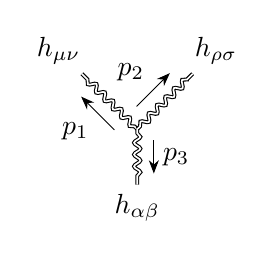
\begin{tikzpicture}[baseline=(o)]
                        \begin{feynhand}
                            \vertex (o) at (0, 0);
                            \vertex (h1) at (-1, 1) {$h_{\mu\nu}$};
                            \vertex (h2) at (1, 1) {$h_{\rho\sigma}$};
                            \vertex (h3) at (0, -1) {$h_{\alpha\beta}$};

                            \propag [graviton] (o) to (h1);
                            \propag [mom = $p_1$, opacity=0] (o) to (h1);
                            \propag [graviton] (o) to (h2);
                            \propag [mom = $p_2$, opacity=0] (o) to (h2);
                            \propag [graviton] (o) to (h3);
                            \propag [mom = $p_3$, opacity=0] (o) to (h3);
                        \end{feynhand}
                    \end{tikzpicture} = \ii V_{{(\mu\nu)(\rho\sigma)(\alpha\beta)}}(p_1, p_2, p_3).
                \end{equation}
                The corresponding expression is too lengthy to be presented here, but it could be found in the reproducible Mathematica notebook \githubsrc[Mathematica\_notebooks/Feynman-rules-for-Vertices-via-xAct.nb].

            \subsubsection{\boldmath Vertices of \texorpdfstring{$\phi$-$\phi$-$h$}{ϕ-ϕ-h} and \texorpdfstring{$\varphi$-$\varphi$-$h$}{φ-φ-h}}

                For the vertices of $\phi$-$\phi$-$h$ and $\varphi$-$\varphi$-$h$, the action of
                \begin{equation}
                    S_{\phi + \varphi} = \int \dd[4]{x} \sqrt{-g} \qty[\calL_\phi + \calL_\varphi]
                \end{equation}
                is considered.
                The Feynman rules for the vertices of $\phi$-$\phi$-$h$ and $\varphi$-$\varphi$-$h$ are derived via the package \textsc{xPert} in $\order{\kappa}$ as
                \begin{minted}[gobble=20, breaklines]{mathematica}
                    ExpandPerturbation[Perturbed[L\[Phi], 1] - Perturbed[L\[Phi], 0]]
                    ExpandPerturbation[Perturbed[L\[CurlyPhi], 1] - Perturbed[L\[CurlyPhi], 0]]
                \end{minted}
                where $\texttt{L}\phi = \sqrt{-g} \calL_\phi$ and $\texttt{L}\varphi = \sqrt{-g} \calL_\varphi$.
                Then the Feynman rules for the vertices of $\phi$-$\phi$-$h$ and $\varphi$-$\varphi$-$h$ read
                \begin{equation}
                    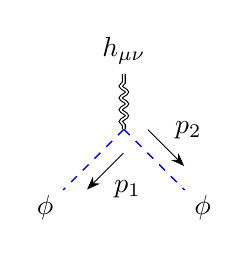
\begin{tikzpicture}[baseline=(o)]
                        \begin{feynhand}
                            \vertex (o) at (0, 0);
                            \vertex (phi1) at (-1, -1) {$\phi$};
                            \vertex (phi2) at (1, -1) {$\phi$};
                            \vertex (h) at (0, 1) {$h_{\mu\nu}$};

                            \propag [scalar, mom=\textcolor{black}{$p_1$}, blue] (o) to (phi1);
                            \propag [scalar, mom=\textcolor{black}{$p_2$}, blue] (o) to (phi2);
                            \propag [graviton] (o) to (h);
                        \end{feynhand}
                    \end{tikzpicture} = -\ii \kappa \qty[p_1^\mu p_2^\nu + p_1^\nu p_2^\mu - \eta^{\mu\nu} \qty(p_1 \cdot p_2 - m_\phi^2)],
                \end{equation}
                and
                \begin{equation}
                    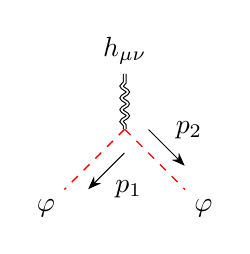
\begin{tikzpicture}[baseline=(o)]
                        \begin{feynhand}
                            \vertex (o) at (0, 0);
                            \vertex (varphi1) at (-1, -1) {$\varphi$};
                            \vertex (varphi2) at (1, -1) {$\varphi$};
                            \vertex (h) at (0, 1) {$h_{\mu\nu}$};

                            \propag [scalar, mom=\textcolor{black}{$p_1$}, red] (o) to (varphi1);
                            \propag [scalar, mom=\textcolor{black}{$p_2$}, red] (o) to (varphi2);
                            \propag [graviton] (o) to (h);
                        \end{feynhand}
                    \end{tikzpicture} = -\ii \kappa \qty[p_1^\mu p_2^\nu + p_1^\nu p_2^\mu - \eta^{\mu\nu} \qty(p_1 \cdot p_2 - m_\varphi^2)].
                \end{equation}

            \subsubsection{\boldmath Vertices of \texorpdfstring{$\phi$-$\phi$-$h$-$h$}{ϕ-ϕ-h-h} and \texorpdfstring{$\varphi$-$\varphi$-$h$-$h$}{φ-φ-h-h}}

                For the vertices of $\phi$-$\phi$-$h$-$h$ and $\varphi$-$\varphi$-$h$-$h$, the action of
                \begin{equation}
                    S_{\phi + \varphi} = \int \dd[4]{x} \sqrt{-g} \qty[\calL_\phi + \calL_\varphi]
                \end{equation}
                is considered.
                The Feynman rules for the vertices of $\phi$-$\phi$-$h$-$h$ and $\varphi$-$\varphi$-$h$-$h$ are derived via the package \textsc{xPert} in $\order{\kappa^2}$ as
                \begin{minted}[gobble=20, breaklines]{mathematica}
                    ExpandPerturbation[Perturbed[L\[Phi], 2] - Perturbed[L\[Phi], 1]]
                    ExpandPerturbation[Perturbed[L\[CurlyPhi], 2] - Perturbed[L\[CurlyPhi], 1]]
                \end{minted}
                The Feynman rules are too lengthy to be presented here but could be found in the reproducible Mathematica notebook \githubsrc[Mathematica\_notebooks/Feynman-rules-for-Vertices-via-xAct.nb].


            \subsubsection{\boldmath Vertices of \texorpdfstring{$\phi$-$\varphi$-$\varphi$}{ϕ-φ-φ}(-\texorpdfstring{$h$}{h})}

                For the vertices of $\phi$-$\varphi$-$\varphi$(-$h$), the action of
                \begin{equation}
                    S_{\phi\varphi^2} = \int \dd[4]{x} \sqrt{-g} \calL_{\phi\varphi^2}
                \end{equation}
                is considered.
                The Feynman rules for the vertices of $\phi$-$\varphi$-$\varphi$(-$h$) are derived via the package \textsc{xPert}, which are given by
                \begin{equation}
                    \begin{tikzpicture}[baseline=(o)]
                        \begin{feynhand}
                            \vertex (o) at (0, 0);
                            \vertex (varphi1) at (-1, -1) {$\varphi$};
                            \vertex (varphi2) at (1, -1) {$\varphi$};
                            \vertex (phi) at (0, 1) {$\phi$};

                            \propag [scalar, blue] (o) to (phi);
                            \propag [scalar, red] (o) to (varphi1);
                            \propag [scalar, red] (o) to (varphi2);
                        \end{feynhand}
                    \end{tikzpicture} = \ii \lambda,
                \end{equation}
                and
                \begin{equation}
                    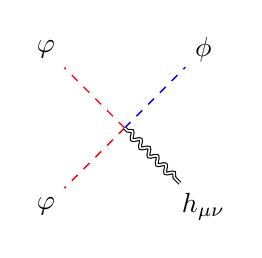
\begin{tikzpicture}[baseline=(o)]
                        \begin{feynhand}
                            \vertex (o) at (0, 0);
                            \vertex (varphi1) at (-1, 1) {$\varphi$};
                            \vertex (varphi2) at (-1, -1) {$\varphi$};
                            \vertex (phi) at (1, 1) {$\phi$};
                            \vertex (h) at (1, -1) {$h_{\mu\nu}$};

                            \propag [scalar, red] (o) to (varphi1);
                            \propag [scalar, red] (o) to (varphi2);
                            \propag [scalar, blue] (o) to (phi);
                            \propag [graviton] (o) to (h);
                        \end{feynhand}
                    \end{tikzpicture} = \ii \kappa \lambda \eta_{\mu\nu}.
                \end{equation}

        \subsection{Propagators and External Legs}
            
            In this note, we do not consider the derivation of the Feynman rules for the propagators and external legs.
            For the scalar fields, the propagators are simply given by \cite[Sec.~10]{Srednicki:2007qs}
            \begin{equation}
                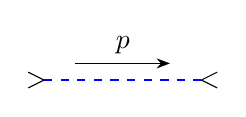
\begin{tikzpicture}[baseline=(phi1)]
                    \begin{feynhand}
                        \vertex (phi1) at (0, 0);
                        \vertex (phi1-1) at (-.2, .1);
                        \vertex (phi1-2) at (-.2, -.1);
                        \vertex (phi2) at (2, 0);
                        \vertex (phi2-1) at (2.2, .1);
                        \vertex (phi2-2) at (2.2, -.1);

                        \propag [scalar, mom=\textcolor{black}{$p$}, blue] (phi1) to (phi2);

                        \draw (phi1-1) -- (phi1) -- (phi1-2);
                        \draw (phi2-1) -- (phi2) -- (phi2-2);
                    \end{feynhand}
                \end{tikzpicture} = \frac{-\ii}{p^2 + m_\phi^2 - \ii 0^+},
            \end{equation}
            and
            \begin{equation}
                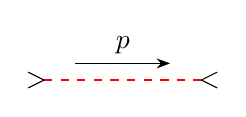
\begin{tikzpicture}[baseline=(phi1)]
                    \begin{feynhand}
                        \vertex (phi1) at (0, 0);
                        \vertex (phi1-1) at (-.2, .1);
                        \vertex (phi1-2) at (-.2, -.1);
                        \vertex (phi2) at (2, 0);
                        \vertex (phi2-1) at (2.2, .1);
                        \vertex (phi2-2) at (2.2, -.1);

                        \propag [scalar, mom=\textcolor{black}{$p$}, red] (phi1) to (phi2);

                        \draw (phi1-1) -- (phi1) -- (phi1-2);
                        \draw (phi2-1) -- (phi2) -- (phi2-2);
                    \end{feynhand}
                \end{tikzpicture} = \frac{-\ii}{p^2 + m_\varphi^2 - \ii 0^+}.
            \end{equation}
            The external legs for scalar fields are always $1$ \cite[Sec.~10]{Srednicki:2007qs}.

            For the graviton, the propagator in the \emph{Feynman gauge} is given by \cite[Eq.~(2.81)]{Basile:2024oms}
            \begin{equation}
                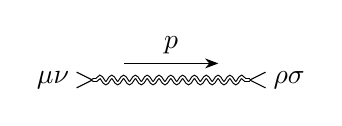
\begin{tikzpicture}[baseline=(h1)]
                    \begin{feynhand}
                        \vertex (h1) at (0, 0);
                        \vertex (h1-1) at (-.2, .1);
                        \vertex (h1-2) at (-.2, -.1);
                        \vertex (h2) at (2, 0);
                        \vertex (h2-1) at (2.2, .1);
                        \vertex (h2-2) at (2.2, -.1);

                        \vertex (h1text) at (-.5, 0) {$\mu\nu$};
                        \vertex (h2text) at (2.5, 0) {$\rho\sigma$};

                        \propag [graviton] (h1) to (h2);
                        \propag [mom=$p$, opacity=0] (h1) to (h2);

                        \draw (h1-1) -- (h1) -- (h1-2);
                        \draw (h2-1) -- (h2) -- (h2-2);
                    \end{feynhand}
                \end{tikzpicture} = \frac{1}{2} \frac{-\ii}{p^2 - \ii 0^+} \qty(\eta_{\mu\rho} \eta_{\nu\sigma} + \eta_{\mu\sigma} \eta_{\nu\rho} - \eta_{\mu\nu} \eta_{\rho\sigma}).
            \end{equation}
            The external legs for the graviton are given by
            \begin{equation}
                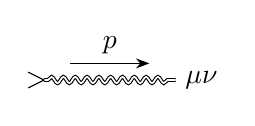
\begin{tikzpicture}[baseline=(h1)]
                    \begin{feynhand}
                        \vertex (h1) at (0, 0);
                        \vertex (h1-1) at (-.2, .1);
                        \vertex (h1-2) at (-.2, -.1);
                        \vertex (h2) at (2, 0) {$\mu\nu$};


                        \propag [graviton] (h1) to (h2);
                        \propag [mom=$p$, opacity=0] (h1) to (h2);

                        \draw (h1-1) -- (h1) -- (h1-2);
                    \end{feynhand}
                \end{tikzpicture} = \varepsilon_{\mu\nu}(\vb{p}, \pm 2),
            \end{equation}
            and
            \begin{equation}
                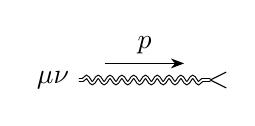
\begin{tikzpicture}[baseline=(h1)]
                    \begin{feynhand}
                        \vertex (h1) at (0, 0) {$\mu\nu$};
                        \vertex (h2) at (2, 0);
                        \vertex (h2-1) at (2.2, .1);
                        \vertex (h2-2) at (2.2, -.1);

                        \propag [graviton] (h1) to (h2);
                        \propag [mom=$p$, opacity=0] (h1) to (h2);

                        \draw (h2-1) -- (h2) -- (h2-2);
                    \end{feynhand}
                \end{tikzpicture} = \varepsilon_{\mu\nu}^*(\vb{p}, \pm 2),
            \end{equation}
            where $\varepsilon_{\mu\nu}(\vb{p}, \pm 2)$ and $\varepsilon_{\mu\nu}^*(\vb{p}, \pm 2)$ are the polarization tensors of the graviton ($\pm 2$ for helicities).
            We do not discuss the details of the polarization tensors here but refer to Ref.~\cite[Sec.~2.2]{Basile:2024oms} for details.
            However, we are interested in the summation over the helicities as \cite[Eq.~(A.6)]{Barman:2023ymn}
            \begin{equation}
                P_{\mu\nu, \rho\sigma} := \sum_{h = \pm 2} \varepsilon_{\mu\nu}(\vb{p}, h) \varepsilon_{\rho\sigma}^*(\vb{p}, h) = \frac{1}{2} \qty(\bar{\eta}_{\mu\rho} \bar{\eta}_{\nu\sigma} + \bar{\eta}_{\mu\sigma} \bar{\eta}_{\nu\rho} - \bar{\eta}_{\mu\nu} \bar{\eta}_{\rho\sigma}),
            \end{equation}
            where
            \begin{equation}
                \bar{\eta}_{\mu\nu} = \eta_{\mu\nu} - \frac{p_\mu r_\nu + r_\mu p_\nu}{p \cdot r}
            \end{equation}
            with $r^\mu$ being an arbitrary null vector for reference.
            Notice that
            \begin{equation}
                q^\alpha P_{\mu\nu, \rho\sigma} \equiv 0 \qfor q = p, r \qand \alpha = \mu, \nu, \rho, \sigma
                \label{eq:transverse-condition}
            \end{equation}
            and
            \begin{equation}
                g^{\mu\nu} P_{\mu\nu, \rho\sigma} = g^{\rho\sigma} P_{\mu\nu, \rho\sigma} = 0,
                \label{eq:traceless-condition}
            \end{equation}
            which means the polarization tensors are transverse and traceless as expected.

    \section{Amplitudes}

        With the Feynman rules we have derived, we could calculate the amplitudes for the processes of interest, where the package \textsc{FeynCalc} \cite{Mertig:1990an, Shtabovenko:2016sxi, Shtabovenko:2020gxv, Shtabovenko:2023idz} is applied.
        In \githubsrc[Mathematica\_notebooks/FeynmanRules.m], the generated Feynman rules are automatically loaded for the calculation of the amplitudes in the following sections.

        \paragraph{Important Note:}
        In \textsc{FeynCalc}, the metric signature is $-2$ instead of $+2$.
        The Feynman rules derived in the previous section should be modified accordingly:
        \begin{minted}[gobble=12, breaklines]{mathematica}
            outputRule = {
                ph1[a_] -> FV[ph1, a], ph2[a_] -> FV[ph2, a], ph3[a_] -> FV[ph3, a],

                p\[Phi]1[a_] -> FV[p\[Phi]1, a], p\[Phi]2[a_] -> FV[p\[Phi]2, a],

                p\[CurlyPhi]1[a_] -> FV[p\[CurlyPhi]1, a],
                p\[CurlyPhi]2[a_] -> FV[p\[CurlyPhi]2, a],

                \[Eta][a_, b_] -> -MT[a, b], FV[p1_, a_] FV[p2_, -a_] -> -SP[p1, p2]
            } // HoldForm;
        \end{minted}

        \subsection{\boldmath \texorpdfstring{$\phi \to \varphi \varphi$}{inflaton → reheaton + reheaton}}

            For the process of $\phi(p) \to \varphi(k_1) + \varphi(k_2)$, the Feynman diagram and the corresponding amplitude are given by
            \begin{equation}
                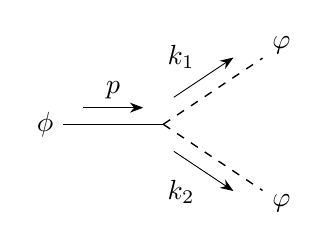
\begin{tikzpicture}[baseline=(phi-varphi-varphi)]
                    \begin{feynhand}
                        \vertex (phi) at (-1.5, 0) {$\phi$};
                        \vertex (varphi1) at (1.5, 1) {$\varphi$};
                        \vertex (varphi2) at (1.5, -1) {$\varphi$};
                        \vertex (phi-varphi-varphi) at (0, 0);

                        \propag [mom=$p$] (phi) to (phi-varphi-varphi);
                        \propag [sca, mom=$k_1$] (phi-varphi-varphi) to (varphi1);
                        \propag [sca, mom'=$k_2$] (phi-varphi-varphi) to (varphi2);
                    \end{feynhand}
                \end{tikzpicture} = \ii \lambda,
            \end{equation}
            The norm squared of the amplitude with the summation over the spins/helicities of final states and the average over the spins/helicities of initial states is then
            \begin{equation}
                \barMsqr[\phi \to \varphi \varphi] = \lambda^2.
            \end{equation}
            Therefore, the decay width of $\phi \to \varphi \varphi$ is given by \cite[Eq.~(49.18)]{ParticleDataGroup:2024cfk}
            \begin{equation}
                \begin{aligned}
                    \Gamma_{\phi \to \varphi \varphi} & = \frac{1}{2 m_\phi} \int \tildedp{k_1} ~ \tildedp{k_2} ~ \twopidelta[4]{p - k_1 - k_2} \frac{\barMsqr[\phi \to \varphi \varphi]}{2} \\
                    & = \frac{\lambda^2}{32 \pi m_\phi^2} \sqrt{m_\phi^2 - 4 m_\varphi^2},
                \end{aligned}
            \end{equation}
            where the factor $1/2$ is due to the identical particles in the final state.
            If $m_\varphi \to 0$, we have
            \begin{equation}
                \Gamma_{\phi \to \varphi \varphi} = \frac{\lambda^2}{32 \pi m_\phi}.
            \end{equation}

        \subsection{\texorpdfstring{\boldmath $\phi + \phi \to h_{\mu\nu} + h_{\rho\sigma}$}{ϕ + ϕ → h\_{µν} + h\_{ρσ}}}

            For the process of $\phi(p_1) + \phi(p_2) \to h_{\mu\nu}(k_1) + h_{\rho\sigma}(k_2)$, the corresponding Feynman diagrams are shown in Fig.~\ref{fig:phi-phi-to-h-h}.

            \begin{figure}[h]
                \centering
                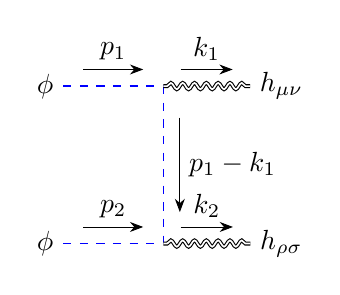
\begin{tikzpicture}
                    \begin{feynhand}
                        \vertex (phi-1) at (-1.5, 1) {$\phi$};
                        \vertex (phi-2) at (-1.5, -1) {$\phi$};
                        \vertex (phi-phi-h-1) at (0, 1);
                        \vertex (phi-phi-h-2) at (0, -1);
                        \vertex (h1) at (1.5, 1) {$h_{\mu\nu}$};
                        \vertex (h2) at (1.5, -1) {$h_{\rho\sigma}$};

                        \propag [scalar, blue, mom=\textcolor{black}{$p_1$}] (phi-1) to (phi-phi-h-1);
                        \propag [scalar, blue, mom=\textcolor{black}{$p_2$}] (phi-2) to (phi-phi-h-2);
                        \propag [scalar, blue, mom=\textcolor{black}{$p_1 - k_1$}] (phi-phi-h-1) to (phi-phi-h-2);
                        \propag [graviton] (phi-phi-h-1) to (h1);
                        \propag [opacity=0, mom=$k_1$] (phi-phi-h-1) to (h1);
                        \propag [graviton] (phi-phi-h-2) to (h2);
                        \propag [opacity=0, mom=$k_2$] (phi-phi-h-2) to (h2);
                    \end{feynhand}
                \end{tikzpicture}
                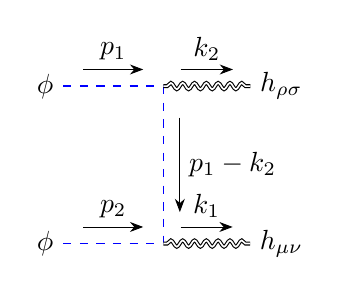
\begin{tikzpicture}
                    \begin{feynhand}
                        \vertex (phi-1) at (-1.5, 1) {$\phi$};
                        \vertex (phi-2) at (-1.5, -1) {$\phi$};
                        \vertex (phi-phi-h-1) at (0, 1);
                        \vertex (phi-phi-h-2) at (0, -1);
                        \vertex (h1) at (1.5, -1) {$h_{\mu\nu}$};
                        \vertex (h2) at (1.5, 1) {$h_{\rho\sigma}$};

                        \propag [scalar, blue, mom=\textcolor{black}{$p_1$}] (phi-1) to (phi-phi-h-1);
                        \propag [scalar, blue, mom=\textcolor{black}{$p_2$}] (phi-2) to (phi-phi-h-2);
                        \propag [scalar, blue, mom=\textcolor{black}{$p_1 - k_2$}] (phi-phi-h-1) to (phi-phi-h-2);
                        \propag [graviton] (phi-phi-h-2) to (h1);
                        \propag [opacity=0, mom=$k_1$] (phi-phi-h-2) to (h1);
                        \propag [graviton] (phi-phi-h-1) to (h2);
                        \propag [opacity=0, mom=$k_2$] (phi-phi-h-1) to (h2);
                    \end{feynhand}
                \end{tikzpicture}
                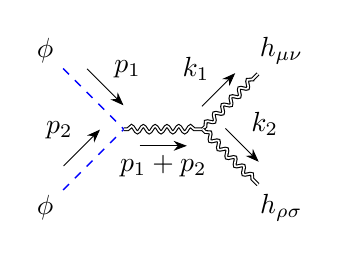
\begin{tikzpicture}
                    \begin{feynhand}
                        \vertex (phi-1) at (-1.5, 1) {$\phi$};
                        \vertex (phi-2) at (-1.5, -1) {$\phi$};
                        \vertex (phi-phi-h) at (-.5, 0);
                        \vertex (h-h-h) at (.5, 0);
                        \vertex (h1) at (1.5, 1) {$h_{\mu\nu}$};
                        \vertex (h2) at (1.5, -1) {$h_{\rho\sigma}$};

                        \propag [scalar, blue, mom=\textcolor{black}{$p_1$}] (phi-1) to (phi-phi-h);
                        \propag [scalar, blue, mom=\textcolor{black}{$p_2$}] (phi-2) to (phi-phi-h);
                        \propag [graviton] (phi-phi-h) to (h-h-h);
                        \propag [opacity=0, mom'=$p_1 + p_2$] (phi-phi-h) to (h-h-h);
                        \propag [graviton] (h-h-h) to (h1);
                        \propag [opacity=0, mom=$k_1$] (h-h-h) to (h1);
                        \propag [graviton] (h-h-h) to (h2);
                        \propag [opacity=0, mom=$k_2$] (h-h-h) to (h2);
                    \end{feynhand}
                \end{tikzpicture}
                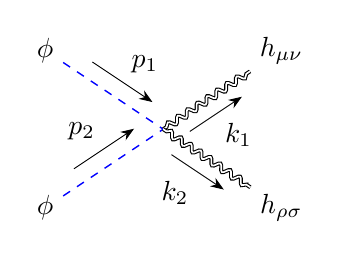
\begin{tikzpicture}
                    \begin{feynhand}
                        \vertex (phi-1) at (-1.5, 1) {$\phi$};
                        \vertex (phi-2) at (-1.5, -1) {$\phi$};
                        \vertex (phi-phi-h-h) at (0, 0);
                        \vertex (h1) at (1.5, 1) {$h_{\mu\nu}$};
                        \vertex (h2) at (1.5, -1) {$h_{\rho\sigma}$};

                        \propag [scalar, blue, mom=\textcolor{black}{$p_1$}] (phi-1) to (phi-phi-h-h);
                        \propag [scalar, blue, mom=\textcolor{black}{$p_2$}] (phi-2) to (phi-phi-h-h);
                        \propag [graviton] (phi-phi-h-h) to (h1);
                        \propag [opacity=0, mom'=$k_1$] (phi-phi-h-h) to (h1);
                        \propag [graviton] (phi-phi-h-h) to (h2);
                        \propag [opacity=0, mom'=$k_2$] (phi-phi-h-h) to (h2);
                    \end{feynhand}
                \end{tikzpicture}
                \caption{Feynman diagrams for $\phi(p_1) + \phi(p_2) \to h_{\mu\nu}(k_1) + h_{\rho\sigma}(k_2)$: $t$-, $u$-, $s$-, and contact channels.}
                \label{fig:phi-phi-to-h-h}
            \end{figure}

            The corresponding amplitudes are calculated in \githubsrc[Mathematica\_notebooks/phi-phi-to-h-h.nb].
            Since the $P_{\mu\nu, \rho\sigma}$ is TT as shown in Eqs.~\eqref{eq:transverse-condition} and \eqref{eq:traceless-condition}, we could make the replacements to simplify the calculations, which are given by
            \begin{equation}
                    k_i \to 0, \qquad p_2 \to -p_1, \qquad \eta_{\mu\nu} \to 0, \qquad \eta_{\rho\sigma} \to 0.
            \end{equation}
            In the \textsc{Wolfram Mathematica} notebook, the \texttt{magicRule} consists of the replacements, which reads
            \begin{minted}[gobble=16, breaklines]{mathematica}
                magicRule = {FV[k1, _] -> 0, FV[k2, _] -> 0, MT[\[Mu], \[Nu]] -> 0, 
                    MT[\[Rho], \[Sigma]] -> 0, MT[\[Mu]C, \[Nu]C] -> 0, 
                    MT[\[Rho]C, \[Sigma]C] -> 0, FV[p2, \[Mu]_] -> -FV[p1, \[Mu]]};
            \end{minted}
            Therefore, the amplitudes are simplified to
            \begin{align}
                \iM[t] & \simeq -\frac{4 \ii \kappa^2}{t - m_\phi^2} p_1^\mu p_1^\nu p_1^\rho p_1^\sigma, \\
                \iM[u] & \simeq -\frac{4 \ii \kappa^2}{u - m_\phi^2} p_1^\mu p_1^\nu p_1^\rho p_1^\sigma, \\
                \iM[s] & \simeq \cdots, \\
                \iM[4] & \simeq \cdots,
            \end{align}
            where the expressions for $\iM[s]$ and $\iM[4]$ are too lengthy to be presented here.
            Please refer to the \textsc{Wolfram Mathematica} notebook for details.
            The norm squared of the amplitudes with the summation over the spins/helicities of all external particles is then
            \begin{equation}
                \sumMsqr[\phi + \phi \to h + h] = \frac{2 \kappa^2}{s^2 \qty(t - m_\phi^2)^2 \qty(s + t - m_\phi^2)^2} \qty[
                    \begin{aligned}
                        m_\phi^{16} - 8 m_\phi^{14} t - 8 m_\phi^2 t^4 (s + t)^3 + t^4 (s + t)^4 \\
                        {} + 4 m_\phi^{12} t (s + 7 t) + 4 m_\phi^4 t^3 (s + t)^2 (s + 7 t) \\
                        {} - 8 m_\phi^{10} t^2 (3 s + 7 t) - 8 m_\phi^6 t^3 (s + t) (3 s + 7 t) \\
                        {} + m_\phi^8 \qty(s^4 + 6 s^2 t^2 + 60 s t^3 + 70 t^4)
                    \end{aligned}
                ].
            \end{equation}
            This lengthy expression could be simplified by considering the non-relativistic (NR) limit or the ultra-relativistic (UR) limit.

            For the NR limit, we have
            \begin{equation}
                s \to 4 m_\phi^2, \qquad t \to -m_\phi^2, \qand u \to -m_\phi^2,
            \end{equation}
            which leads to $\calM_t \calM_i^* = \calM_i^* \calM_t = \calM_u \calM_i^* = \calM_i^* \calM_u = 0$ for $i$ being $t$, $u$, $s$ or $4$.
            The non-vanishing terms are
            \begin{align}
                \Msqr[s] & = 18 \kappa^4 m_\phi^4, \\
                \Msqr[4] & = 32 \kappa^4 m_\phi^4, \\
                \calM_s \calM_4^* + \calM_4 \calM_s^* & = -48 \kappa^4 m_\phi^4,
            \end{align}
            which are consistent with Eq.~(A3) of Ref.~\cite{Choi:2024ilx}.

            In the UR limit, we have $m_\phi \to 0$, which leads to
            \begin{equation}
                \sumMsqr[\phi + \phi \to h + h] = \frac{2 \kappa^2 t^2 u^2}{s^2},
            \end{equation}
            which is consistent with Eq.~(25) of Ref.~\cite{Ghiglieri:2022rfp}\footnote{Notice that $\kappa = \MPl^{-1}$ in this note, while $\kappa = 2 \MPl^{-1}$ in Ref.~\cite{Ghiglieri:2022rfp}.}.
    
    \clearpage
    \appendix
    \numberwithin{equation}{section}

    \section{Conventions}\label{app:convention}

        Here, we list the conventions used in this note.

        \subsection{Spacetime: Metric and Curvature}
        
            We use the Greek indices $\mu, \nu, \ldots$ for spacetime indices and the Latin indices $i, j, \ldots$ for spatial indices.
            For $D$-dimensional spacetime, we have the spacetime indices run from $0$ to $D - 1$, and the spatial indices run from $1$ to $D - 1$, where $0$ is the time index and other indices are spatial indices.
            Usually, we consider $D = 4$ spacetime dimensions.

            In four-dimensional spacetime, the metric signature is chosen to be $+2$, \eg,
            \begin{equation}
                \eta_{\mu\nu} = \mqty(\dmat[0]{-1, +1, +1, +1})
            \end{equation}
            for the Minkowski metric.

            The covariant and contravariant vectors in spacetime are denoted as $A_\mu$ and $A^\mu$, respectively.
            They are related by the metric $g_{\mu\nu}$ as
            \begin{equation}
                A_\mu \equiv g_{\mu\nu} A^\nu \qand A^\mu \equiv g^{\mu\nu} A_\nu,
            \end{equation}
            where $g^{\mu\nu}$ is the inverse of $g_{\mu\nu}$, \ie,
            \begin{equation}
                g^{\mu\nu} g_{\nu\rho} = \delta\indices{^\mu_\rho} \qand g_{\mu\nu} g^{\nu\rho} = \delta\indices{_\mu^\rho}.
            \end{equation}
            Here we adopt the Einstein summation convention, where indices appearing twice with one as a superscript and the other as a subscript are summed over.
            Without specification, the Einstein summation convention is applied throughout this note.

            The Riemman curvature tensor for the spacetime is defined as \cite[Eq.~(3.4)]{Carroll:2004st}
            \begin{equation}
                R\indices{^\rho_{\sigma\mu\nu}} := \partial_\mu \Gamma\indices{^\rho_{\nu\sigma}} - \partial_\nu \Gamma\indices{^\rho_{\mu\sigma}} + \Gamma\indices{^\rho_{\mu\lambda}} \Gamma\indices{^\lambda_{\nu\sigma}} - \Gamma\indices{^\rho_{\nu\lambda}} \Gamma\indices{^\lambda_{\mu\sigma}},
            \end{equation}
            where $\Gamma\indices{^\rho_{\mu\nu}}$ is the Christoffel symbol defined as \cite[Eq.~(3.1)]{Carroll:2004st}
            \begin{equation}
                \Gamma\indices{^\rho_{\mu\nu}} := \frac{1}{2} g^{\rho\sigma} \qty(\partial_\mu g_{\nu\sigma} + \partial_\nu g_{\mu\sigma} - \partial_\sigma g_{\mu\nu}).
            \end{equation}
            The Ricci tensor and scalar curvature are then given by \cite[Eqs.~(3.144) and (3.146)]{Carroll:2004st}
            \begin{align}
                R_{\mu\nu} & := R\indices{^\rho_{\mu\rho\nu}}, \\
                R & := g^{\mu\nu} R_{\mu\nu}.
            \end{align}
            The Einstein tensor is defined as \cite[Eq.~(3.151)]{Carroll:2004st}
            \begin{equation}
                G_{\mu\nu} := R_{\mu\nu} - \frac{1}{2} g_{\mu\nu} R,
            \end{equation}
            and the Einstein field equation is then \cite[Eq.~(4.100)]{Carroll:2004st}
            \begin{equation}
                G_{\mu\nu} + \Lambda g_{\mu\nu} = \kappa^2 T_{\mu\nu},
            \end{equation}
            where $\Lambda$ is the cosmological constant, $\kappa^2 = 8 \pi \GN$ \cite[Eq.~(2.1)]{Basile:2024oms} with $\GN = 6.70883(15) \timestento{-39} ~ \GeV^{-2}$ being the Newton's constant \cite{ParticleDataGroup:2024cfk}, and $T_{\mu\nu}$ is the energy-momentum tensor.

            This convention is also adopted in MTW's \textit{Gravitation} \cite{Misner:1973prb}, which is known as $(+ + +)$ convention.

        \subsection{Natural Units and (reduced) Planck Mass}

            The natural unit systems are given by 
            \begin{equation}
                c = \hbar = \kB = \varepsilon_0 = 1,
            \end{equation}
            where $c$ is the speed of light in vacuum, $\hbar$ is the reduced Planck constant, $\kB$ is the Boltzmann constant, and $\varepsilon_0$ is the vacuum permittivity.
            We have the vacuum magnetic permeability $\mu_0 = 1$ as well in the natural unit systems since $c^2 = (\varepsilon_0 \mu_0)^{-1}$.
            

            The Planck mass is defined as
            \begin{equation}
                \mPl := \frac{1}{\sqrt{\GN}},
            \end{equation}
            In this note, the reduced Planck mass is widely used, which is defined as
            \begin{equation}
                \MPl := \frac{1}{\sqrt{8 \pi \GN}} \equiv \frac{\mPl}{\sqrt{8 \pi}}.
                \label{eq:reduced-Planck-mass}
            \end{equation}

        \subsection{Kinematics}

            The four-momentum $p$ is defined as $p^\mu = (E, \vb{p})$, where $E$ is the energy and $\vb{p}$ is the spatial momentum.
            The on-shell condition is given by $p^2 = -m^2$ for metric signature $+2$.

            In the $n \to m$ scattering process $p_1 + p_2 + \cdots + p_n \to k_1 + k_2 + \cdots + k_m$ with $p_i$'s and $k_j$'s the four-momenta of the incoming and outgoing particles, respectively, the four-momentum conservation is given by
            \begin{equation}
                p_1 + p_2 + \cdots + p_n = k_1 + k_2 + \cdots + k_m.
            \end{equation}
            We denote the masses of the particles as $m_i$'s for $p_i$'s and $\frakm_j$'s for $k_j$'s, \ie,
            \begin{equation}
                \left\{
                    \begin{aligned}
                        p_i^2 & = -m_i^2, \\
                        k_j^2 & = -\frakm_j^2.
                    \end{aligned}
                \right.
            \end{equation}
            
            The Lorentz-invairant phase space element for the four-momentum $p$ is defined as
            \begin{equation}
                \tildedp{p} := \frac{\dd[3]{\vb{p}}}{\twopi[3] 2 E},
            \end{equation}
            where $p = \qty(E, \vb{p})$ and $p^2 = -E^2 + \vb{p}^2 = -m^2$.

            For the $2 \to 2$ scattering process $p_1 + p_2 \to k_1 + k_2$, the Mandelstam variables are defined as
            \begin{equation}
                \begin{aligned}
                    s & := -(p_1 + p_2)^2 \equiv -(k_1 + k_2)^2, \\
                    t & := -(p_1 - k_1)^2 \equiv -(p_2 - k_2)^2, \\
                    u & := -(p_1 - k_2)^2 \equiv -(p_2 - k_1)^2.
                \end{aligned}
                \label{eq:s-t-u}
            \end{equation}
            For the $1 \to 3$ scattering process $p_1 \to k_1 + k_2 + k_3$, the Mandelstam variables are defined as
            \begin{equation}
                \begin{aligned}
                    s & := -(p_1 - k_3)^2 \equiv -(k_1 + k_2)^2, \\
                    t & := -(p_1 - k_1)^2 \equiv -(k_2 + k_3)^2, \\
                    u & := -(p_1 - k_2)^2 \equiv -(k_1 + k_3)^2.
                \end{aligned}
            \end{equation}

    \clearpage
    \printbibliography[heading=bibintoc]
\end{document}
